\documentclass[12pt]{article}

\usepackage[english]{babel}
\usepackage[margin=1in]{geometry}
\usepackage[utf8x]{inputenc}
\usepackage{amsmath}
\usepackage{graphicx}
\usepackage{verbatim}
\usepackage{placeins}

\setlength{\parskip}{1pc}
\setlength{\parindent}{0pt}


\title{Scratch Interfaces: Reliably Classifying Scratch Audio Data}
\author{Oliver Song}

\begin{document}
\maketitle

\section{Introduction}

In this report the problem of recognizing scratch gestures with a single microphone is addressed. This is an interesting problem both because the modality itself and its hardware requirements. Scratching sounds are very unique. They produce high frequency, high amplitude noise within the medium they are applied to. Additionally, almost any surface can be used as a medium, such as a wall, a table, a clipboard, your pants, or even your arm. Sound is propagated through these surfaces extremely far and with remarkably little distortion and loss of quality. Using a single microphone, a scratch on the other side of a surface, from one end of a room to the other, can be heard clearly. While input strength may vary, and inputting with a finger nail may be uncomfortable on some surfaces or to some people, it still presents an incredibly versatile medium for inputting gestures. This was also an interesting subject because I personally have never learned about or worked with signal processing in any capacity. Learning about convolutions, filters, and in general how to manipulate signals has been an eye opening experience. On top of that, this was an interesting opportunity to try to use HMMs we were taught to use throughout the class in a novel situation.

\subsection{Related Work}

In a paper by Chris Harrison and Scott E. Hudson, the concept of single microphone scratch gesture input was first introduced. A modified stethoscope was used as the microphone, and ``X", ``Zero", ``i", ``F", and ``Y" gestures were tested. Their gesture recognition seemed to be based not only on amplitude but also on frequency. The assumption they made was that when the scratch was slower, it produced lower frequency noise, and when it was faster, it produced higher frequency noise.

\section{Data collection methods}

Throughout the project, the same microphone was used. Two different methods of input were used: fingernail input and screwdriver input. Each scratch was recorded for 2 seconds at 8000hz in mono.

\subsection{Materials}
The microphone that was chosen was the P-007 High Quality Contact Mic. Pickup, shown in Figure 1.

\begin{figure}[h!]
\centering
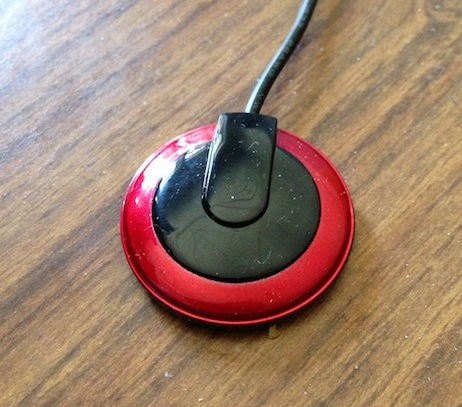
\includegraphics[scale=0.5]{microphone.jpg}
\caption{The microphone, a P-007 High Quality Contact Mic. Pickup}
\end{figure}

It is also worth mentioning that the microphone was only meant to go straight into a speaker amplifier, as it is normally attached to some kind of instrument to amplify its sound. In order to use it as a recording device for my computer, I had to use a Mono-to-3.5mm converter piece, as well as a male-to-male 3.5mm cable. These two pieces of converting equipment, shown in Figure 2, were not particularly high quality, and so could have contributed to noise and weak signal.

\begin{figure}[h!]
\centering
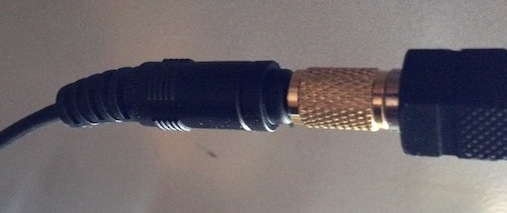
\includegraphics[scale=0.5]{connection.jpg}
\caption{Convertor used for the microphone}
\end{figure}

The medium that was used was the top of my desk, which can also be seen in Figure 1. It is a polished wooden veneer, which is not particularly hard, but adequately transfers sound. A better alternative would have been the wall or the floor.

The gestures that were used throughout the project changed dramatically. Gestures with similar amplitude profiles were discarded in favor of more varied gestures. The final 6 gestures that were used in the project can be fund in Appendix B.

\FloatBarrier

\subsection{Finger input}
Initially, I started testing fingernail input. The sound recorded by the microphone was so low that I couldn't actually see it on the plot. I had to boost the mic input by 30 decibels to get a reasonable reading. However, noise was significant. Unfortunately  this was a byproduct of having used cheap materials. Fortunately, this provides a good base line for measuring scratches in very noisy conditions. If better equipment was available, this would be analogous to the case of trying to classify scratches with a fan or AC unit attached to the medium.

An example of a scratches produced by this method of input can be seen in Figure 3.

\begin{figure}[h!]
\centering
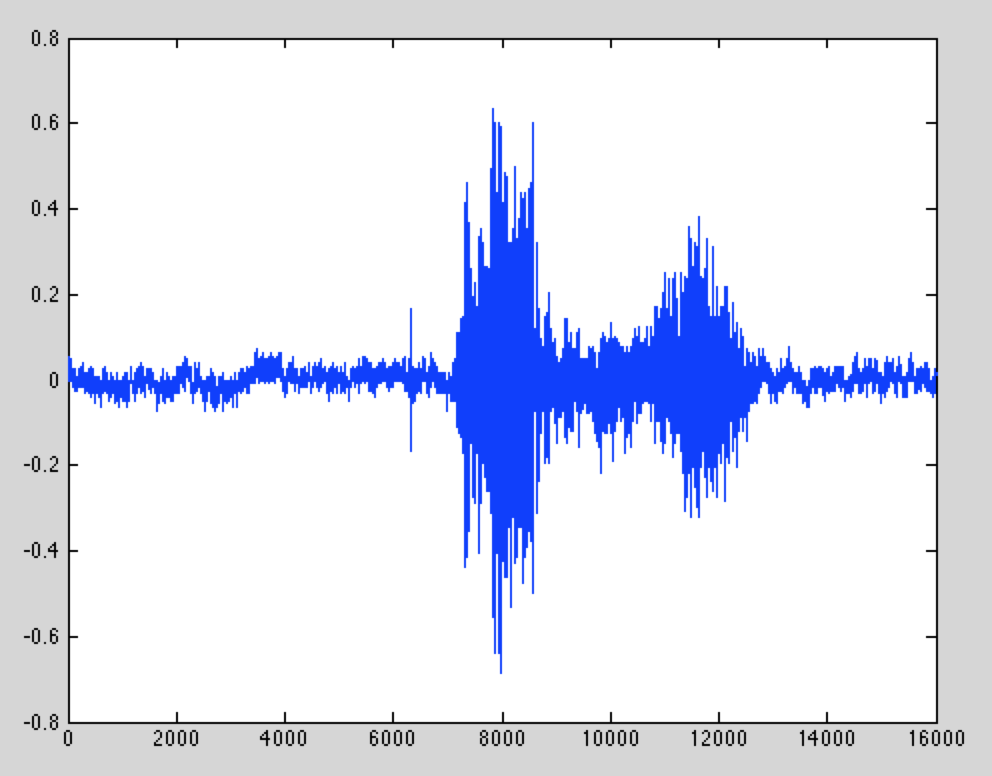
\includegraphics[scale=0.7]{noisy.png}
\caption{Noisy data}
\end{figure}

\FloatBarrier
\subsection{Screwdriver input}
To compensate for suboptimal equipment, instead of boosting the signal, I needed to simply create a better source of noise. Instead of a fingernail, I used a screwdriver. Screwdrivers, or any kind of metal, is much harder than a fingernail, and creates a much stronger signal when scratching. The difference was dramatic, and I did not have to boost the screwdriver signal at all. This led to almost no noise; an ideal set of data.

An example of the ``hard" scratches I produced can be seen in Figure 4.

\begin{figure}[h!]
\centering
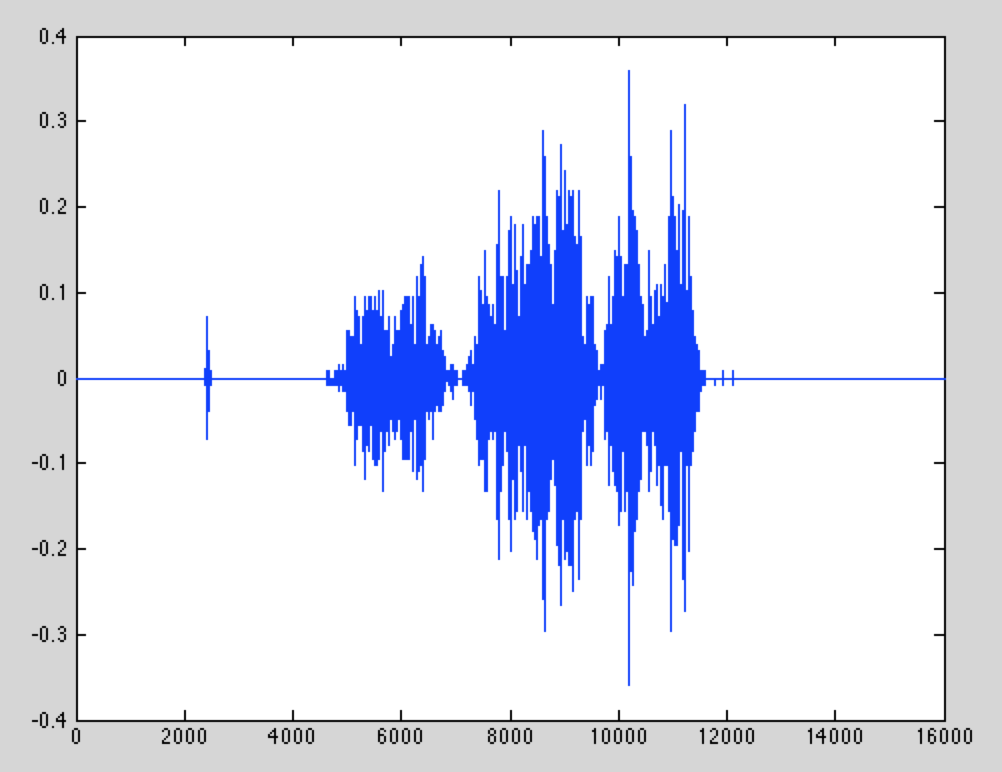
\includegraphics[scale=0.7]{hard.png}
\caption{``Hard" ideal data}
\end{figure}

\FloatBarrier

\section{Data filtering methods}

Initially, I thought that scratches were only very high frequency noises. I thought I would only need to apply a high-pass filter to remove noise and run the HMM classifier and be done. However, scratches are actually composed of a broad spectrum of frequencies, including the lower range. This can be seen in Figure 5. In removing the low range of frequencies to take out noise, I was actually taking out the scratch noise as well.

\begin{figure}[h!]
\centering
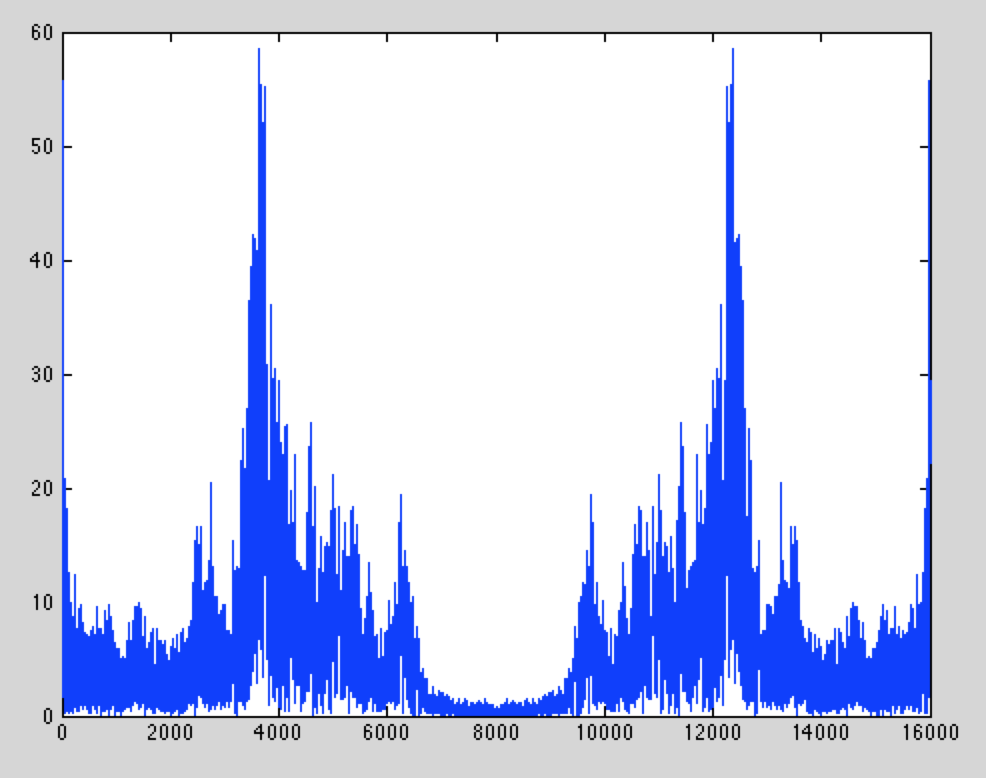
\includegraphics[scale=0.7]{fft.png}
\caption{Fourier transform of some sample data}
\end{figure}

I decided to classify based only on amplitude. This restricted the number of possible gestures, but was still manageable.

I took the absolute value of the signal, then cut values left and right of the signal that were below a threshold. This gave me a set of signals of around the same length. I then found the average length of the signals and scaled each signal to that average length. Now I had a set of same-length signals.

At this point I tried analyze the data with the HMM classifier, but it classified terribly. It classified no better than perfectly randomly, scoring 12.5\% (I had 8 gestures at the time). I thought it might be that the signal was still too noisy, so I applied a gaussian filter to all the data. However, this did not solve the problem.

Eventually, I discovered ``envelope" functions, which take an approximation for the maxima or minima of a signal. This is exactly what I needed. An example is shown in Figure 6. I took the upper envelope of all the signal data, and the HMM classifier's performance increased (37\%).

\begin{figure}[h!]
\centering
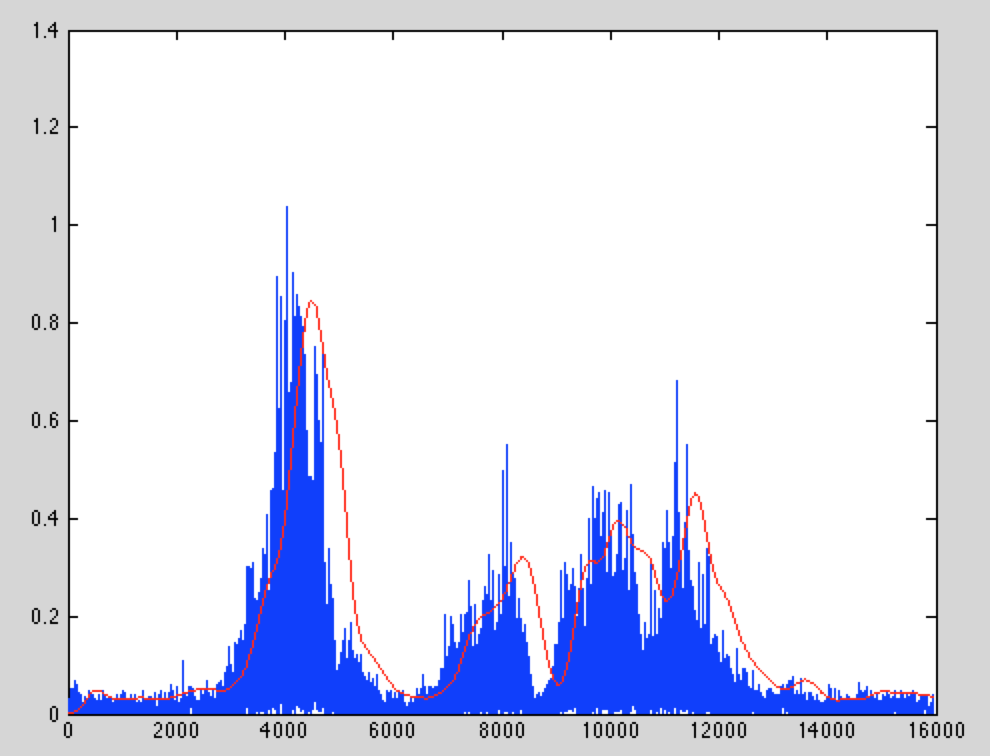
\includegraphics[scale=0.7]{enveloped.png}
\caption{Upper envelope of data}
\end{figure}
\FloatBarrier

Finally, I realized I needed to normalize the data, since certain signals simply overpowered others. After normalizing all of the signals, I saw a massive increase in classification accuracy. An example of a normalized enveloped signal can be seen in Figure 7.

\begin{figure}[h!]
\centering
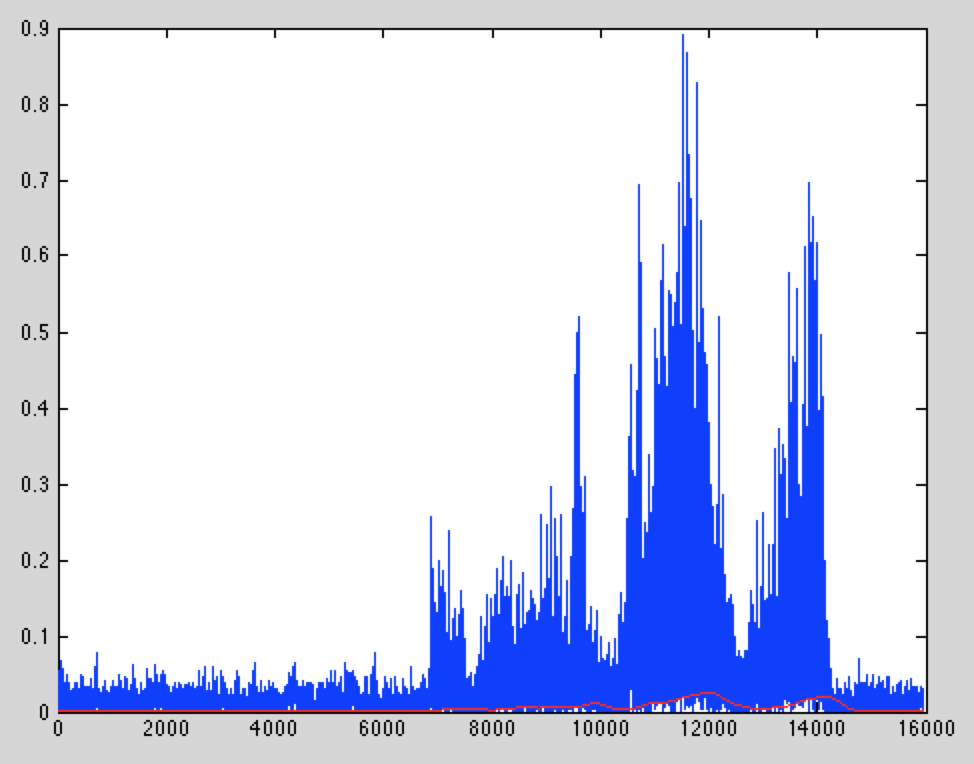
\includegraphics[scale=0.7]{normalized.png}
\caption{Normalized upper envelope}
\end{figure}

\FloatBarrier

\section{Classification methods}


\subsection{BNT and HMM}
I tried using the methods that were presented in Project 3, with the Kinect, but it proved to be extremely inaccurate. After some initial trouble, I realized it would be much easier to just put my data in the same format as the Kinect data, and experiment\_hmm ran flawlessly for me. It started at 12.5\% accuracy, and as I added in improvements to filtering gradually improved to around 40\% accuracy. Unfortunately, this is still abysmal.

\subsection{Overlap classifier}

Since using the BNT package wasn't panning out for me, I decided to work on a custom classification algorithm. I knew that I would need to find a measure for how much two signals were alike. I immediately thought of hamming distance, the nearest neighbor classifier that we made for the very same Kinect project. But how do you implement hamming distance for audio signals? You could take the envelope function result of the two signals and subtract them, but that leaves some negative values and weird things happen.

I decided to multiply the two compared data series together, and find the total of resulting series. This effectively gave me a score for how much the two signals overlapped, and for any non overlapping segments, the resultant signal would be zero.

Implementing this, I immediately saw results of over 50\% accuracy.

\subsubsection{Shifting}
I realized that some of the signals simply didn't match up, because errors in the left/right cutoff of my data filtering. Since they were not necessarily aligned, they would not score well on the overlap classifier. So, I shifted the compared signal with the comparing signal by 1/10 their length. I padded zeroes of 1/20 their length on both sides, then compared at every 10 points up until the end of the signal. This algorithm can be seen in section 9.5. This led to about a 10\% accuracy boost.

\subsubsection{Normalization}

The real kicker was when I discovered that one type of scratch was outweighing all the others, and therefore skewing results unfavorably. I realized that some scratches simply had more {\bf net amplitude}. To fix this, I took each signal and divided it by its 2-norm. The matlab 2-norm of a one dimensional vector is its normalization. The intuition behind this is to scale all signals to the same net amplitude so that they're weighted equally when doing overlap classification.

This led to a 30-40\% accuracy boost.

\section{Results}

\subsection{Running HMM on filtered noisy data}
I first ran experiment\_hmm on the filtered noisy data I initially collected. This led to everything being classified as one gesture, giving it the same score as a perfectly random choice, or 12.5\%. This was discouraging.

\begin{figure}[h!]
\centering
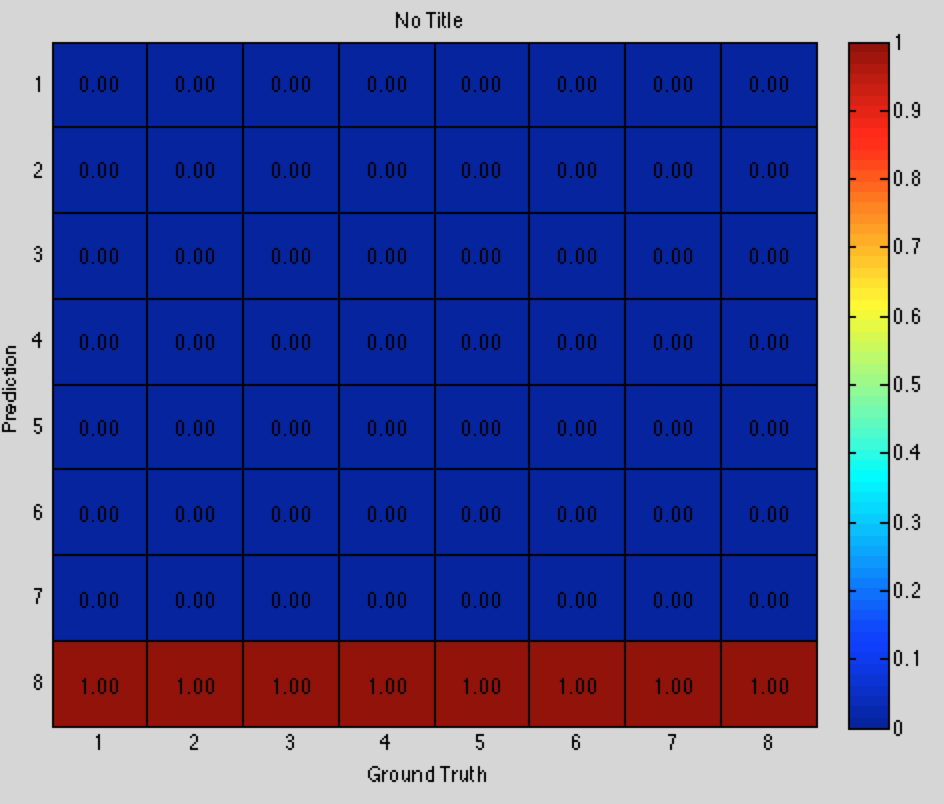
\includegraphics[scale=0.6]{raw.png}
\caption{Filtered noisy raw data HMM run}
\end{figure}

\FloatBarrier
\subsection{Running HMM on filtered good data}
I thought that maybe the signals were too noisy. As a result, I collected the noise free screwdriver scratches, and reran experiment\_hmm. This resulted in about an 18\% accuracy. Better than random, but still terrible.

\begin{figure}[h!]
\centering
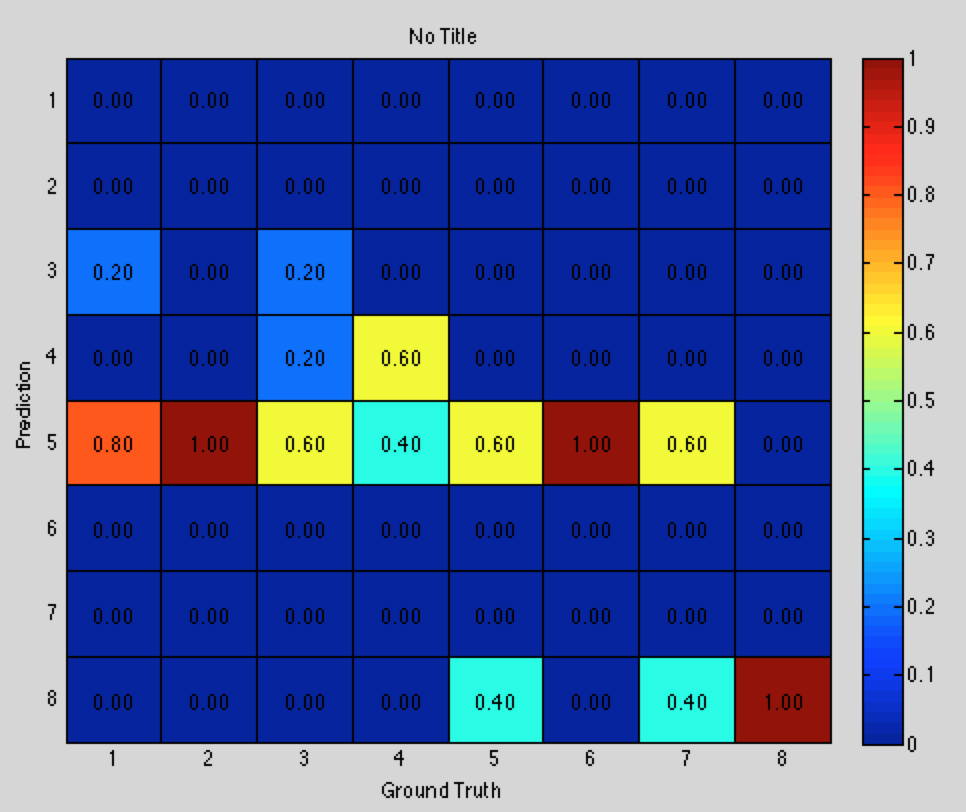
\includegraphics[scale=0.6]{filteredhmm.png}
\caption{Filtered good raw data HMM run}
\end{figure}

\FloatBarrier
\subsection{Running HMM on enveloped good data}
I discovered envelope functions, and reran experiment\_hmm on the upper envelope of the good filtered data. I ended up with an accuracy of about 37\%. Now we're getting somewhere!

\begin{figure}[h!]
\centering
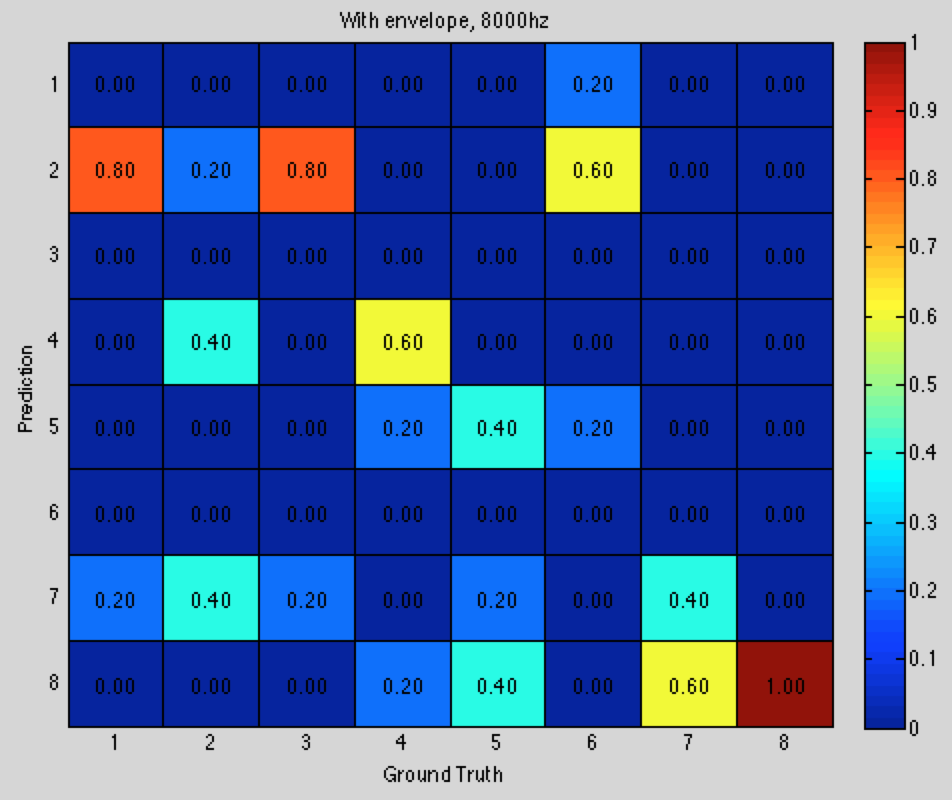
\includegraphics[scale=0.6]{envelopedhmm.png}
\caption{Enveloped filtered good data}
\end{figure}

\FloatBarrier
\subsection{Running Overlap classifier on enveloped good data}
I got tired of not knowing what experiment\_hmm was doing and why it was performing so poorly, so I created the overlap classifier. Running on the same set of data as in 5.3, it saw about a 55\% accuracy.

\begin{figure}[h!]
\centering
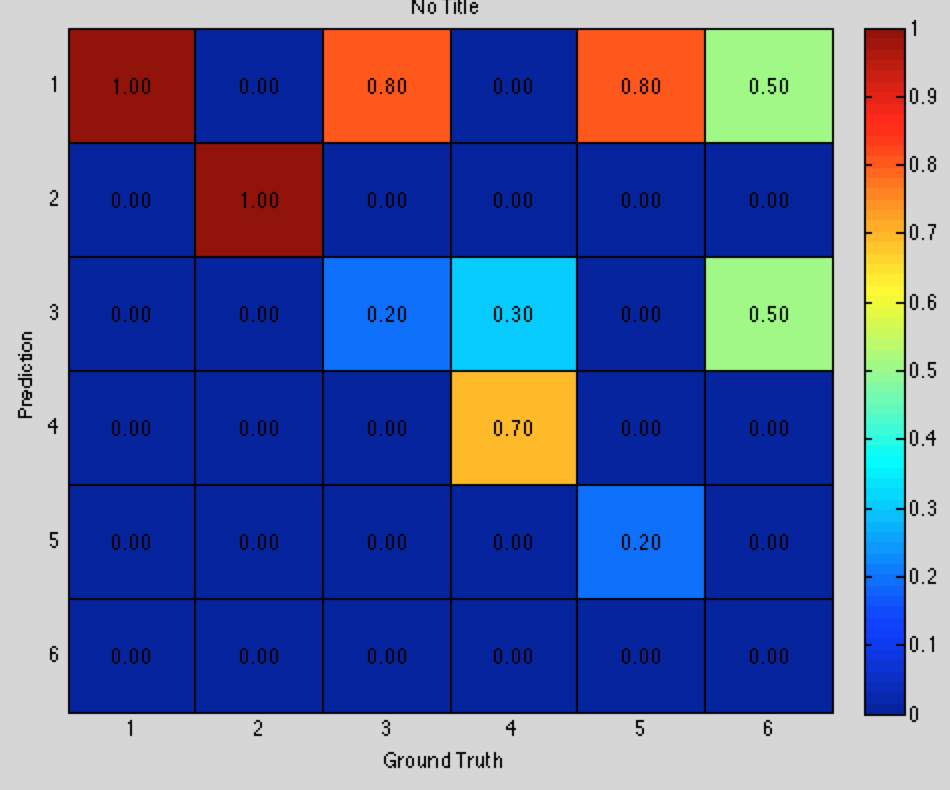
\includegraphics[scale=0.6]{overlapinit.png}
\caption{Overlap classifier on enveloped good data}
\end{figure}

\FloatBarrier
\subsection{Running overlap classifier on normalized shifted enveloped noisy data}
Finally, I discovered normalization, and upon rerunning the overlap classifier, obtained 80-90\% accuracy on noisy data.

\begin{figure}[h!]
\centering
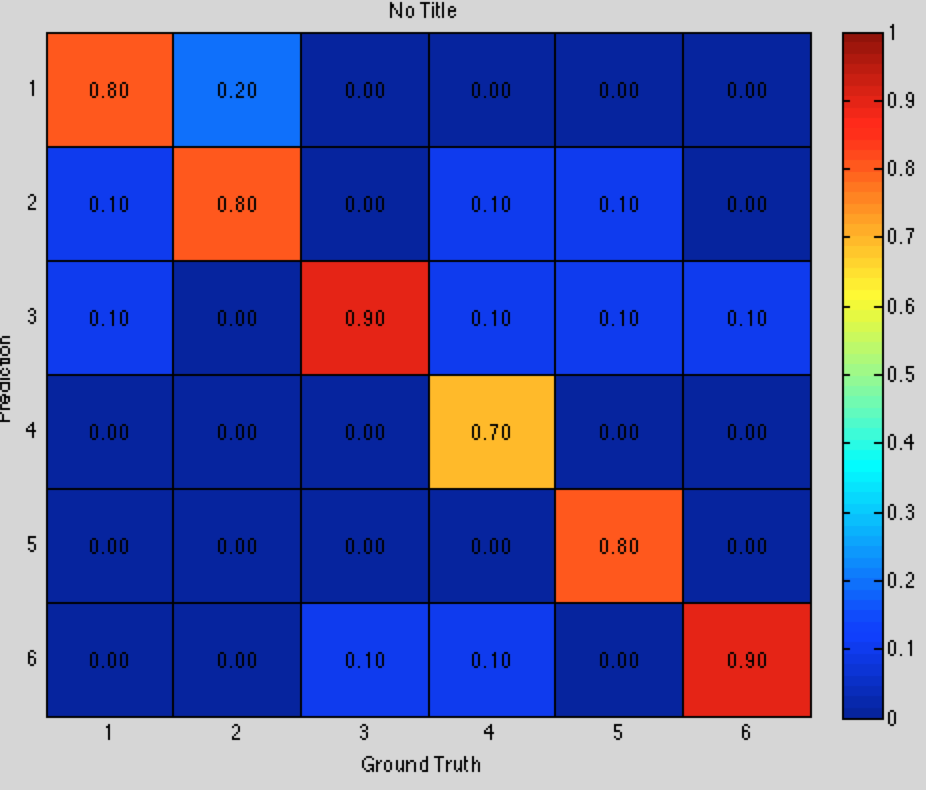
\includegraphics[scale=0.6]{finalnoisy.png}
\caption{Overlap classifier with normalized noisy data}
\end{figure}


\FloatBarrier
\subsection{Running overlap classifier on normalized shifted enveloped good data}
The classifier performed astronomically well on noise free data. 100\% accurate!

\begin{figure}[h!]
\centering
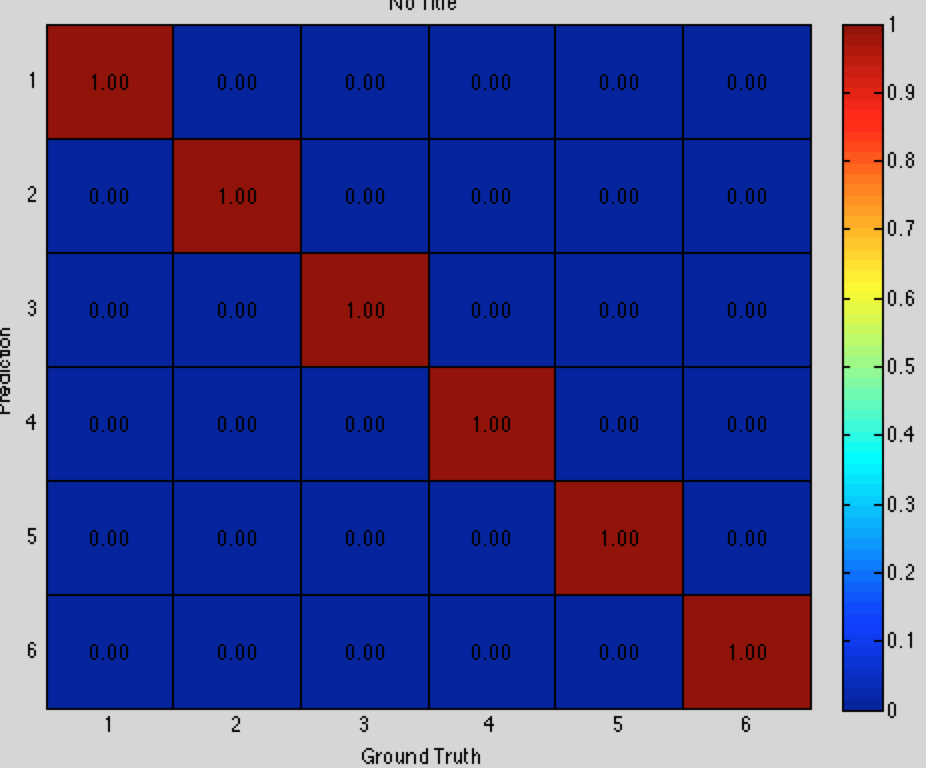
\includegraphics[scale=0.6]{finalhard.png}
\caption{Overlap classifier with normalized good data}
\end{figure}

\FloatBarrier
\section{Discussion}

Going through this project has been a phenomenal learning process. Having never done anything with signal processing before, I learned quite a lot. I believe that, given more time, I could have made the HMM package work correctly with this kind of data and gotten even better classification with noisy data. However, the classifier I managed to create can already be used real-time for very accurate classification. It can classify a single gesture in 200 milliseconds, with 90\% accuracy in a noisy environment. I could even have used better equipment and more types of mediums, as well as types of gestures.

Something that is intriguing to me now that I have a bit more understanding is the prospect of integrating frequency information in to the classification. As mentioned before, a previous project managed to do this. I could treat frequency profile and amplitude as two different modalities, and test different levels of fusion on them. Unfortunately, my understand of HMMs and signals was too weak to be able to complete this in the given time, but this would make for some interesting further work.

\section{Conclusion}

In this report I addressed the problem of recognizing scratch gestures with a single microphone. I started out with a perfectly random classifier, and as I learned more about signals, incrementally increased classification accuracy until I achieved 100\% accuracy on good data. Key realizations along the way were taking the upper envelope of the data and normalizing all data. In the future, integrating frequency profile data is a definite possibility, making it an actual "multimodal" interface. For reasonable circumstances, my algorithm can quickly classify scratches in a noisy environment with 80-90\% accuracy, and 100\% accuracy in a noise free environment.

\section{Acknowledgements}

I'd would like to thank Professor Davis for the time he has invested in 6.835 this semester. The concepts that were introduced in lecture not only helped me grasp some important concepts about multimodal interfaces but were also useful in giving me context and background information while I was doing working on this project.

Additionally, I'd like to thank my Teaching Assistant, Yale Song, for the time he put in to making and grading projects, and responding so quickly to any problems I had in this and previous projects.

\section{Appendix A: Code}

\subsection{build\_dataset.m}

\begin{verbatim}
function [scratch_data] = build_dataset()
    num_gestures = 10;
    gesture_types = {'triangle','square','loop','X','zigzag','balloon'};
    recObj = audiorecorder;
    record_length = 2;
    
    % builds the dataset.
    scratch_data = cell(1, numel(gesture_types));
    for i=1:numel(scratch_data)
        scratch_data{i}.label = gesture_types(i);
        scratch_data{i}.data = cell(1, num_gestures);
    end
    
    % make the audio recordings and store them.
    for i=1:numel(gesture_types)
        for j=1:num_gestures
            disp(strcat('Scratch for: ',gesture_types(i),'#',int2str(j)))
            % 2 seconds should be enough
            recordblocking(recObj, record_length);
            disp('End of Recording.');
            scratch_data{i}.data{j} = getaudiodata(recObj);
        end
    end
end
\end{verbatim}

\subsection{filter\_data.m}

\begin{verbatim}
function [filtered_data] = filter_data(scratch_data)
    filtered_data = scratch_data;
    domains= zeros(numel(scratch_data)*numel(scratch_data{1}.data),1);
    disp('trimming and averaging')
    for i=1:numel(scratch_data)
        for j=1:numel(scratch_data{i}.data)
            current = scratch_data{i}.data{j};
            % trim data of small values left and right
            i1 = find(current>0.01, 1, 'first');
            i2 = find(current>0.01, 1, 'last');
            segment = current(i1:i2);
            f_seg = segment;
            % figure out the average domain
            domains((i-1)*numel(scratch_data{i}.data)+j) = length(f_seg);
            filtered_data{i}.data{j} = f_seg;
        end
    end
    disp('scaling everything to the same domain')    
    avg_domain = ceil(mean(mean(domains)));
    for i=1:numel(scratch_data)
        for j=1:numel(scratch_data{i}.data)
        % scale data to average domain
            filtered_data{i}.data{j} = interpft(filtered_data{i}.data{j},avg_domain);
        end
    end
end
\end{verbatim}

\subsection{format\_data.m}

\begin{verbatim}

function [formatted] = format_data(filtered)
    formatted = cell(1, numel(filtered));
    for i=1:numel(formatted)
       formatted{i} = cell(1,numel(filtered{i}.data));
    end
    for i=1:numel(formatted)
        for j=1:numel(formatted{i})
            formatted{i}{j} = abs(filtered{i}.data{j})';
        end
    end
end

\end{verbatim}

\subsection{envelope.m}

\begin{verbatim}
function [enveloped] = envelope(data)
    enveloped = data;
    b = fir1(700, 1/8000);
    for i=1:numel(data)
        for j=1:numel(data{i})
            enveloped{i}{j} = 3*filter(b,1,data{i}{j});
        end
    end
    for i=1:numel(enveloped)
        for j=1:numel(enveloped{i})
            enveloped{i}{j} = enveloped{i}{j} / norm(enveloped{i}{j},2);
        end
    end
end
\end{verbatim}

\subsection{classify\_dat.m}

\begin{verbatim}

% classify using highest overlap

function [Ystar, Ytrue] = classify_dat(data)
    Ystar = zeros(1,numel(data)*numel(data{1}));
    Ytrue = zeros(1,numel(data)*numel(data{1}));
    for i=1:numel(data)
        for j=1:numel(data{i})
            Ystar((i-1)*numel(data{i})+j) = classify_one(data{i}{j}, data);
            Ytrue((i-1)*numel(data{i})+j) = i;
        end
    end
    confmat = build_confmat(Ystar, Ytrue);
    plot_confmat(confmat);
    accuracy = sum(Ystar==Ytrue)/numel(Ytrue);
    fprintf('Accuracy: %d',accuracy);
end

function [ highest_probability ] = classify_one( to_check, data)
    scores = zeros(1,numel(data));
    for i=1:numel(data)
        intermediate = zeros(1,numel(data{i}));
        for j=1:numel(data{i})
            intermediate(1,j) = compare_one(to_check,data{i}{j});
        scores(1,i) = mean(intermediate);
        end
    end
    [ maxval, highest_probability ] = max(scores);
end

function [ score ] = compare_one( to_check, compare_against )
    % pad PADDING zeros on either size of compare against
    % run PADDING times and find the maximum score
    padding = 1000;
    padded = padarray(compare_against,[0 padding]);
    scores = zeros(1,padding*2);
    for i=1:padding*2
        blah = sum(to_check.*padded(i:i+length(compare_against)-1));
        scores(i) = blah;
    end
    score = max(scores);
end

\end{verbatim}


\section{Appendix B: Gestures}

\begin{figure}[h!]
\centering
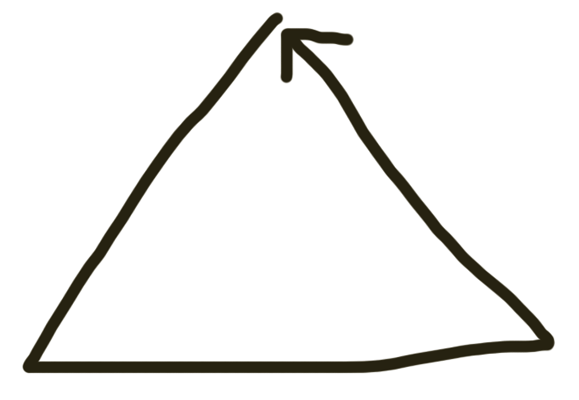
\includegraphics[scale=0.4]{triangle.png}
\caption{Triangle gesture}
\end{figure}

\begin{figure}[h!]
\centering
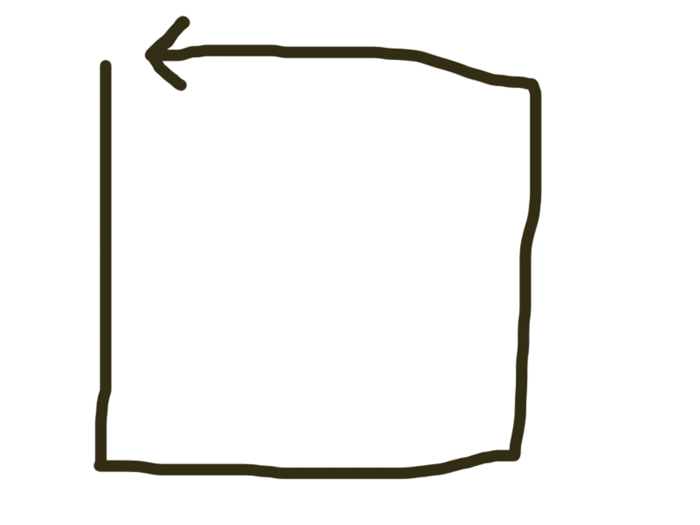
\includegraphics[scale=0.4]{square.png}
\caption{Square gesture}
\end{figure}

\begin{figure}[h!]
\centering
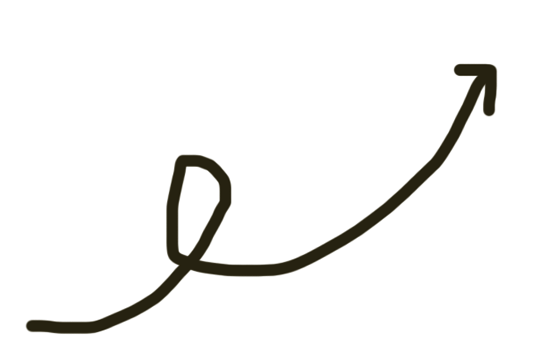
\includegraphics[scale=0.4]{loop.png}
\caption{Loop gesture}
\end{figure}

\begin{figure}[h!]
\centering
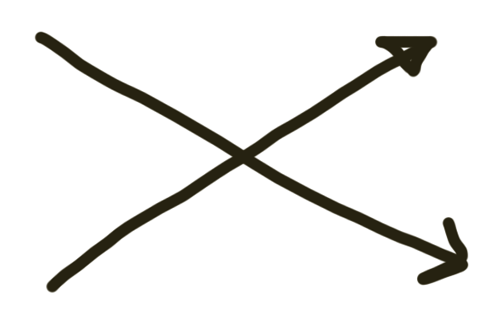
\includegraphics[scale=0.4]{X.png}
\caption{X gesture}
\end{figure}

\begin{figure}[h!]
\centering
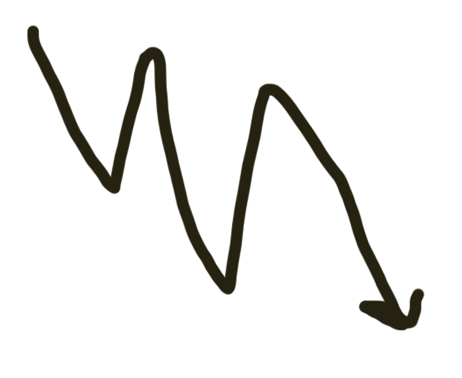
\includegraphics[scale=0.4]{zigzag.png}
\caption{Zigzag gesture}
\end{figure}

\begin{figure}[h!]
\centering
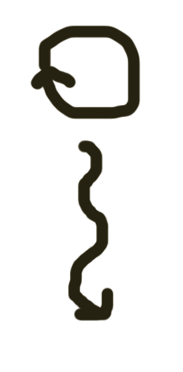
\includegraphics[scale=0.4]{balloon.png}
\caption{Balloon gesture}
\end{figure}

\FloatBarrier

\section{References}
\begin{itemize}
\item[1] Harrison, Chris and Hudson, Scott E. Scratch Input: Creating Large, Inexpensive, Unpowered and Mobile finger Input Surfaces. In Proceedings of the 21st Annual ACM Symposium on User interface Software and Technology. UIST '08. ACM, New York, NY. 205-208.
\item[2] Steve Mann, Ryan Janzen and Raymond Lo, ``Hyperacoustic instruments: Computer-controlled instruments that are not electrophones", Proc. International IEEE conference (ICME 2008), Hannover, Germany, June 23-26, 2008.

\item[3] Halajian, Gary, and John Wang. ``Gesture Recognition Based on Scratch Inputs." Cit.cornell.edu. Cornell, 26 Apr. 2009. Web. 17 May 2013.
\end{itemize}
\end{document}